\documentclass[11pt,a4paper]{article}

\usepackage[utf8]{inputenc}
\usepackage[T1]{fontenc}
\usepackage[english]{babel}
\usepackage{graphicx}
\usepackage{amsmath}
\usepackage{amssymb}
\usepackage{booktabs}
\usepackage{siunitx}
\usepackage[margin=2.5cm]{geometry}
\usepackage[hidelinks]{hyperref}
\usepackage{caption}
\captionsetup{labelfont=bf}
\usepackage{float}
\usepackage{chemformula}

\graphicspath{{../figures/}}

\title{
    \large Warsaw University of Technology \\
    Faculty of Power and Aeronautical Engineering \\[1cm]
    \rule{\linewidth}{0.5pt}\\[0.4cm]
    \LARGE \textbf{Effect of Hydrogen Enrichment on Methane--Air Combustion:\\
    Laminar Flame Speed, Ignition Delay and NO\textsubscript{x} Emissions}\\[0.2cm]
    \rule{\linewidth}{0.5pt}\\[0.5cm]
    \large Computer Methods in Combustion -- Project Report
}

\author{Bartosz Cuper 313182}
\date{June 2026}

\begin{document}

\maketitle
\thispagestyle{empty}
\newpage

\begin{abstract}
Blending hydrogen into natural-gas fuel streams is one of the short-term options considered for reducing the carbon
intensity of existing gas infrastructure. However, hydrogen and methane differ substantially in their reactivity,
diffusivity and adiabatic flame temperature, so even moderate H\textsubscript{2} addition can change the
operability and emissions of a combustion system in non-obvious ways. In this project, the GRI-Mech 3.0 chemical
kinetic mechanism is used together with the Cantera software package to study how the hydrogen molar fraction in a
\ch{CH4}/\ch{H2} fuel blend, $X_{H2} \in [0,1]$, affects (i) the adiabatic flame temperature and equilibrium
NO\textsubscript{x}/\ch{CO} emissions, (ii) the laminar flame speed $S_L$ of freely propagating premixed flames, and (iii) the
ignition delay time $\tau$ of a constant-volume adiabatic reactor. Results show that hydrogen enrichment increases
the adiabatic flame temperature and equilibrium NO\textsubscript{x} monotonically, increases the laminar flame speed by up to
a factor of six at $X_{H2}=1$, and reduces the ignition delay by one to two orders of magnitude at typical
auto-ignition temperatures, with a qualitatively different (non-monotonic) pressure dependence for pure hydrogen
compared to pure methane. The results are discussed in the context of practical hydrogen-blending limits for
combustion equipment.
\end{abstract}
\newpage

\tableofcontents

\newpage

%======================================================================
\section{Introduction}
%======================================================================

Natural gas combustion remains one of the dominant sources of energy for power generation, industrial heat and
domestic heating. In the transition towards lower-carbon energy systems, blending hydrogen into existing natural
gas networks and burners has been proposed as a relatively low-cost intermediate step, since it can reuse a large
part of the existing pipeline and combustion infrastructure \cite{donohoe2014}. The hydrogen fraction that can be
tolerated by a given system, however, is limited by changes in the combustion characteristics of the fuel blend.

Hydrogen and methane differ strongly in their combustion-relevant properties:
\begin{itemize}
    \item \textbf{Reactivity}: \ch{H2} oxidation proceeds through the very fast \ch{H + O2 -> OH + O} branching
    reaction, giving \ch{H2}/air mixtures laminar flame speeds roughly six to eight times higher than \ch{CH4}/air
    mixtures, and ignition delay times that are orders of magnitude shorter at the same temperature.
    \item \textbf{Heating value}: on a mass basis, hydrogen has a lower heating value (LHV) of approximately
    \SI{120}{MJ/kg}, about 2.4 times that of methane (\SI{50}{MJ/kg}), but on a volumetric basis hydrogen contains
    roughly three times less energy per unit volume.
    \item \textbf{Flame temperature and NO\textsubscript{x}}: the higher adiabatic flame temperature of hydrogen-enriched
    mixtures tends to increase thermal NO\textsubscript{x} formation via the Zeldovich mechanism \cite{zeldovich1946}.
\end{itemize}

The goal of this project is to quantify these effects for a \ch{CH4}/\ch{H2}/air system using detailed chemical
kinetics, spanning the full blending range from pure methane ($X_{H2}=0$) to pure hydrogen ($X_{H2}=1$), where
$X_{H2}$ is the molar fraction of hydrogen in the fuel (i.e. the fuel composition is
$(1-X_{H2})\,\ch{CH4} + X_{H2}\,\ch{H2}$). Specifically, three complementary numerical studies are carried out:

\begin{enumerate}
    \item \textbf{Chemical equilibrium}: adiabatic flame temperature $T_{ad}$ and equilibrium concentrations of
    \ch{NO}, \ch{NO2} and \ch{CO} as a function of equivalence ratio $\phi$ and $X_{H2}$.
    \item \textbf{Laminar flame speed}: one-dimensional freely-propagating premixed flame simulations giving
    $S_L(\phi, X_{H2})$ and its pressure dependence, as well as the flame temperature and species structure.
    \item \textbf{Ignition delay}: zero-dimensional constant-volume adiabatic reactor simulations giving the
    auto-ignition delay time $\tau(T_0, p_0, X_{H2})$.
\end{enumerate}

All simulations use the GRI-Mech 3.0 reaction mechanism \cite{gri30} (53 species, 325 reactions) through the
Cantera 3.2 Python interface \cite{cantera}.

%======================================================================
\section{Literature Review}
%======================================================================

The effect of hydrogen addition on the combustion properties of methane--air (and more generally natural-gas--air)
mixtures has been studied extensively, both experimentally and numerically.

Di Sarli and Di Benedetto \cite{disarli2007} measured and computed the laminar burning velocity and Markstein length
of \ch{H2}/\ch{CH4}/air premixed flames over a wide range of hydrogen fractions and equivalence ratios. They found
that the laminar burning velocity increases monotonically and increasingly steeply with the hydrogen content, with
the strongest relative increase occurring above approximately 50\% \ch{H2} by volume in the fuel -- a trend that is
reproduced qualitatively by the present simulations (Section~\ref{sec:flame_speed}).

Hermanns et al. \cite{hermanns2010} carried out a systematic experimental and modelling study of the laminar burning
velocity of \ch{CH4} + \ch{H2} + \ch{O2} + \ch{N2} flames as a function of unburned gas temperature, equivalence
ratio and hydrogen fraction, providing one of the most complete datasets used for validation of kinetic mechanisms
(including GRI-Mech) in this composition space.

Donohoe et al. \cite{donohoe2014} investigated ignition delay times and laminar flame speeds of natural-gas/hydrogen
blends at engine-relevant elevated pressures, both experimentally (in a shock tube and rapid compression machine)
and numerically. Their results show that hydrogen addition substantially reduces the ignition delay time, and that
the pressure dependence of the ignition delay can differ qualitatively between methane-rich and hydrogen-rich
mixtures because of the competition between the chain-branching reaction \ch{H + O2 -> OH + O} and the pressure-dependent
chain-terminating reaction \ch{H + O2 + M -> HO2 + M}. This competition is discussed further in
Section~\ref{sec:ignition} in the context of the pressure scan results obtained here.

The GRI-Mech 3.0 mechanism \cite{gri30} used in this work was developed and optimized primarily for natural-gas
combustion (methane, with \ch{C2} chemistry and NO\textsubscript{x} sub-mechanism), but it also includes the core
\ch{H2}/\ch{O2} chemistry and is commonly used as a baseline mechanism for \ch{CH4}/\ch{H2} blend studies, as in
\cite{disarli2007,hermanns2010,donohoe2014}.

%======================================================================
\section{Model Description}
%======================================================================

\subsection{Chemical kinetic mechanism and fuel definition}

All simulations use the GRI-Mech 3.0 mechanism \cite{gri30} (\texttt{gri30.yaml} in Cantera), which includes 53
species and 325 elementary reactions, and contains a NO\textsubscript{x} sub-mechanism (thermal/Zeldovich, prompt and
\ch{N2O}-intermediate routes) needed to predict \ch{NO} and \ch{NO2} formation.

The fuel is a binary blend of methane and hydrogen, parametrized by the hydrogen molar fraction in the fuel,
$X_{H2} \in [0,1]$:
\begin{equation}
    \text{Fuel} = (1-X_{H2})\,\ch{CH4} + X_{H2}\,\ch{H2}
\end{equation}
so that $X_{H2}=0$ corresponds to pure methane and $X_{H2}=1$ to pure hydrogen. The oxidizer is air, represented as
$\ch{O2}:1,\ \ch{N2}:3.76$ (molar). For a given equivalence ratio $\phi$, Cantera's
\texttt{set\_equivalence\_ratio} method is used to determine the fuel/air ratio relative to the stoichiometric
ratio, defined in the usual way as
\begin{equation}
    \phi = \frac{(n_{\text{fuel}}/n_{\text{O}_2})}{(n_{\text{fuel}}/n_{\text{O}_2})_{\text{stoich}}}
\end{equation}
For the global reactions
\begin{align}
    \ch{CH4 + 2 O2 -> CO2 + 2 H2O} \\
    \ch{H2 + 1/2O2 -> H2O}
\end{align}
the stoichiometric oxygen requirement of the blend is $2(1-X_{H2}) + \tfrac{1}{2}X_{H2}$ mol \ch{O2} per mol fuel,
which is computed automatically by Cantera from the mechanism's elemental composition. All simulations start from a
fresh, unburned mixture at the specified initial temperature $T_0$ and pressure $p_0$.

The fuel-blend lower heating value (LHV), used to put the energy density of the blends into context, was computed
from the molar enthalpies of the unburned fuel and the fully oxidized products (\ch{CO2} and \ch{H2O}, with
\ch{H2O} assumed gaseous, i.e. LHV) at \SI{298}{K}:
\begin{equation}
    \text{LHV} = \frac{ n_{fuel}\,\bar{h}_{fuel} + n_{O_2}\,\bar{h}_{O_2} - n_{CO_2}\,\bar{h}_{CO_2} - n_{H_2O}\,\bar{h}_{H_2O} }{M_{fuel}}
\end{equation}
where $\bar{h}$ are molar enthalpies obtained from the GRI-Mech thermodynamic data and $M_{fuel}$ is the molar mass
of the fuel blend.

\subsection{Chemical equilibrium model (adiabatic flame temperature, NO\textsubscript{x}/\ch{CO})}

The adiabatic flame temperature and the equilibrium product composition are obtained by equilibrating the unburned
mixture at constant enthalpy and pressure (\texttt{gas.equilibrate("HP")} in Cantera), which solves for the chemical
equilibrium state reachable adiabatically from the given reactants:
\begin{equation}
    H(T_{ad}, p, \mathbf{Y}_{eq}) = H(T_0, p, \mathbf{Y}_0)
\end{equation}
where $\mathbf{Y}_0$ and $\mathbf{Y}_{eq}$ are the reactant and equilibrium product mass-fraction vectors,
respectively. This gives the thermodynamic upper bound on the flame temperature and the equilibrium concentrations
of all 53 species, including \ch{NO}, \ch{NO2} and \ch{CO}, without requiring any information about reaction rates.
All equilibrium calculations are performed at $T_0=\SI{300}{K}$, $p_0=\SI{1}{atm}$.

\subsection{Laminar premixed flame model (1D)}

The laminar flame speed and flame structure are computed with Cantera's \texttt{FreeFlame} class, which solves the
steady, one-dimensional governing equations for a freely-propagating premixed flame in a coordinate system attached
to the flame:
\begin{align}
    \text{Continuity:} \quad & \dot{m} = \rho u = \text{const} \\
    \text{Species:} \quad & \dot{m}\frac{dY_k}{dx} = -\frac{d(\rho Y_k V_k)}{dx} + \dot{\omega}_k W_k \\
    \text{Energy:} \quad & \dot{m} c_p \frac{dT}{dx} = \frac{d}{dx}\left(\lambda \frac{dT}{dx}\right)
    - \sum_k \rho Y_k V_k c_{p,k}\frac{dT}{dx} - \sum_k \dot{\omega}_k h_k W_k
\end{align}
where $\dot{m}$ is the (eigenvalue) mass flux, $Y_k$ the species mass fractions, $V_k$ the diffusion velocities,
$\dot{\omega}_k$ the net production rates and $h_k$ the species enthalpies. The mass-flux eigenvalue, evaluated at
the cold inlet, gives the laminar flame speed $S_L = \dot{m}/\rho_{unburned}$ (\texttt{flame.velocity[0]} in
Cantera).

Mixture-averaged transport properties are used. The domain width is set to \SI{0.03}{m} and an adaptive grid is
used, with refinement controlled by \texttt{set\_refine\_criteria(ratio=3, slope=0.1, curve=0.2)}, which limits the
maximum ratio between adjacent grid spacings and bounds the change in solution slope and curvature between grid
points. The flame is solved with Cantera's damped Newton solver using the \texttt{auto=True} continuation strategy
(\texttt{flame.solve(loglevel=0, auto=True)}), starting from an initial guess and progressively refining the mesh
and relaxing transport/diffusion terms until convergence. All flame simulations use unburned conditions
$T_0=\SI{300}{K}$ unless otherwise stated.

\subsection{Ignition delay model (0D constant-volume reactor)}
\label{sec:ignition_model}

Auto-ignition is modelled using a homogeneous, constant-volume, adiabatic batch reactor\linebreak
(\texttt{IdealGasReactor} coupled to a \texttt{ReactorNet}). The reactor state evolves according to the
species and energy conservation equations for a closed, constant-volume system:
\begin{align}
    \frac{dY_k}{dt} &= \frac{\dot{\omega}_k W_k}{\rho} \\
    \frac{dT}{dt} &= -\frac{1}{\rho c_v}\sum_k u_k \dot{\omega}_k W_k
\end{align}
The reactor is initialized at the desired $(T_0, p_0, \phi, X_{H2})$ state and integrated forward in time. The
ignition delay time $\tau$ is defined as the time at which the temperature rise rate $dT/dt$ reaches its maximum,
i.e. the steepest part of the temperature trace, computed numerically as
$\tau = \arg\max_t \left( dT/dt \right)$ using \texttt{numpy.gradient} on the stored $(t, T)$ trace. A case is
considered "non-igniting" within the simulated time window (and reported as not-a-number) if the total temperature
rise is less than \SI{400}{K}.

This single-stage definition of $\tau$ is appropriate for the present mixtures, which under the conditions studied
show a single dominant thermal runaway. It would, however, not resolve two-stage ignition behaviour (a distinct
low-temperature heat-release stage followed by the main ignition event), which can occur for larger hydrocarbons
but is not significant for \ch{CH4}/\ch{H2} blends in the temperature range studied here.

%======================================================================
\section{Results and Discussion}
%======================================================================

\subsection{Adiabatic flame temperature and equilibrium emissions}
\label{sec:equilibrium}

Figure~\ref{fig:tad_phi} shows the adiabatic flame temperature $T_{ad}$ as a function of equivalence ratio $\phi$
for six hydrogen blend fractions $X_{H2} \in \{0, 0.2, 0.4, 0.6, 0.8, 1.0\}$. For every blend, $T_{ad}$ peaks
slightly on the rich side of stoichiometric ($\phi \approx 1.0$--$1.1$), which is the well-known result of the
balance between increasing heat release and the dissociation of \ch{CO2}/\ch{H2O} at very high temperatures. The
peak temperature increases monotonically with $X_{H2}$:

\begin{table}[H]
\centering
\caption{Maximum adiabatic flame temperature for each fuel blend.}
\label{tab:tad_max}
\begin{tabular}{ccc}
\toprule
$X_{H2}$ & $\phi$ at $T_{ad,max}$ & $T_{ad,max}$ [K] \\
\midrule
0.0 & 1.02 & 2233.2 \\
0.2 & 1.02 & 2243.3 \\
0.4 & 1.05 & 2258.0 \\
0.6 & 1.05 & 2280.5 \\
0.8 & 1.05 & 2318.2 \\
1.0 & 1.08 & 2396.3 \\
\bottomrule
\end{tabular}
\end{table}

Going from pure methane to pure hydrogen increases the maximum adiabatic flame temperature by about
\SI{163}{K} (2233.2~K $\rightarrow$ 2396.3~K), and the equivalence ratio of the peak shifts slightly toward the
rich side as the hydrogen fraction increases. This is consistent with the higher adiabatic flame temperature of
hydrogen-air flames reported in the literature \cite{disarli2007,hermanns2010}.

\begin{figure}[H]
    \centering
    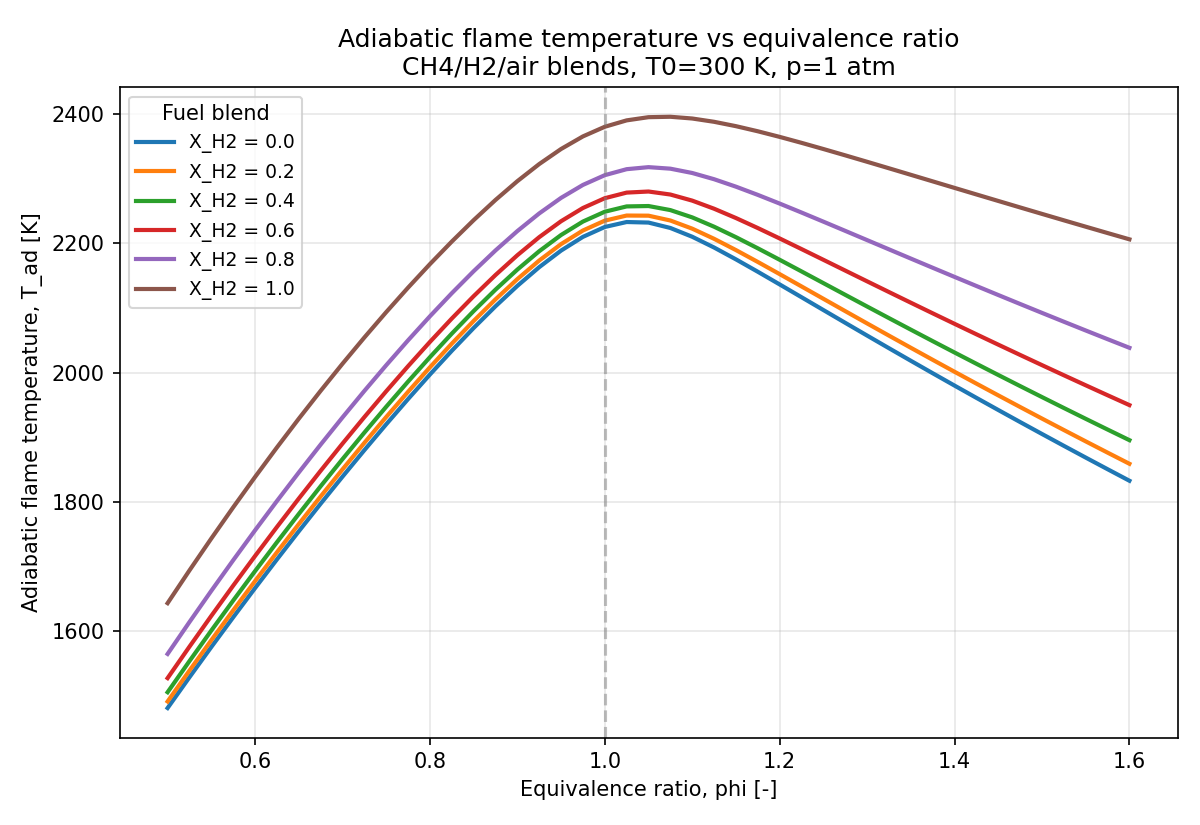
\includegraphics[width=0.85\textwidth]{01_Tad_vs_phi.png}
    \caption{Adiabatic flame temperature vs equivalence ratio for \ch{CH4}/\ch{H2}/air blends ($T_0=\SI{300}{K}$, $p=\SI{1}{atm}$).}
    \label{fig:tad_phi}
\end{figure}

Figure~\ref{fig:nox_phi} shows the equilibrium NO\textsubscript{x} (\ch{NO}+\ch{NO2}) mole fraction versus $\phi$. As
expected from Zeldovich-mechanism thermal \ch{NO} formation, NO\textsubscript{x} peaks under slightly lean conditions
($\phi \approx 0.8$--$0.9$), where the combination of high temperature and excess \ch{O2} availability maximizes
the thermal \ch{NO} formation rate (equilibrium), and decreases sharply for rich mixtures where free \ch{O2} is
depleted. At $\phi=1.0$, increasing $X_{H2}$ from 0 to 1 increases equilibrium NO\textsubscript{x} from
\SI{1888.6}{ppm} to \SI{2529.5}{ppm}, an increase of about 34\%, tracking the increase in $T_{ad}$.

\begin{figure}[H]
    \centering
    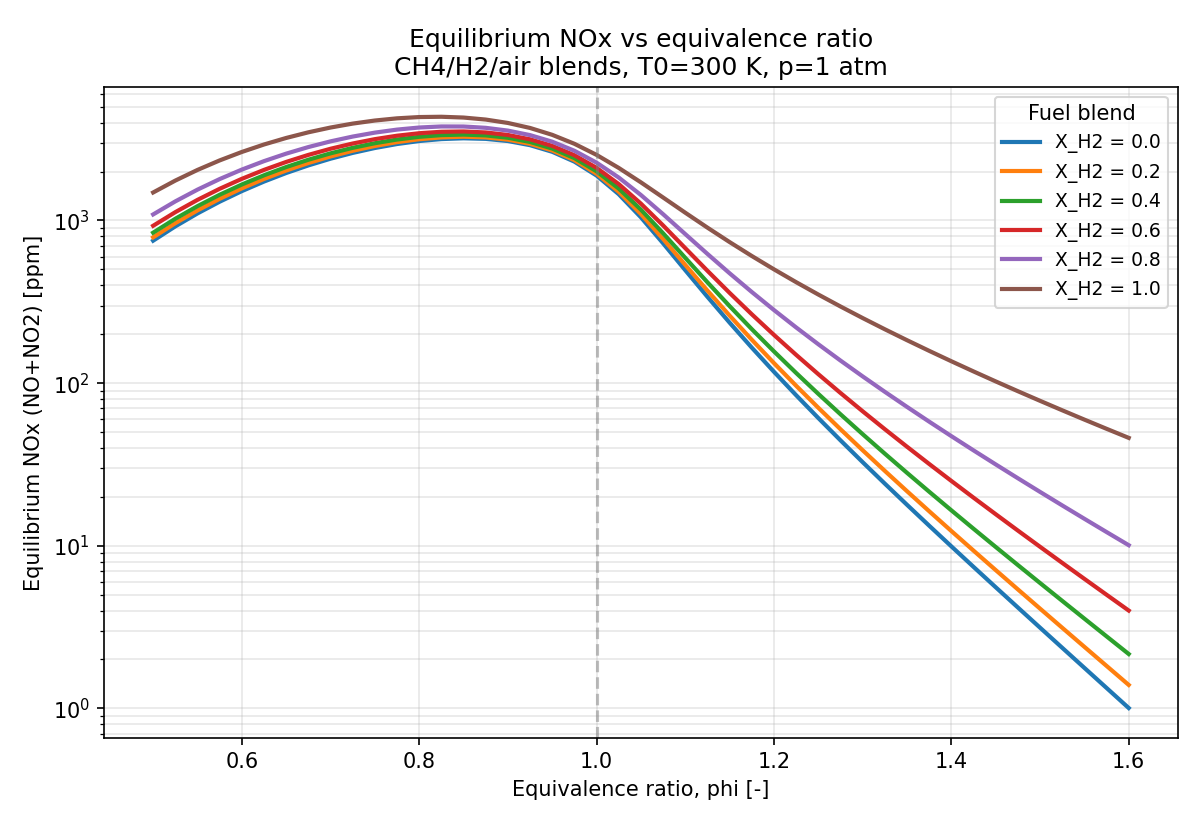
\includegraphics[width=0.85\textwidth]{02_equilibrium_NOx_vs_phi.png}
    \caption{Equilibrium NO\textsubscript{x} (NO + NO\textsubscript{2}) vs equivalence ratio for \ch{CH4}/\ch{H2}/air blends.}
    \label{fig:nox_phi}
\end{figure}

Figure~\ref{fig:co_phi} shows the equilibrium \ch{CO} mole fraction versus $\phi$. \ch{CO} is negligible for lean
and near-stoichiometric mixtures but rises by orders of magnitude for rich mixtures ($\phi>1$), as incomplete
oxidation becomes thermodynamically favoured once the available \ch{O2} is insufficient to fully oxidize the fuel
carbon to \ch{CO2}. For a fixed $\phi$, increasing $X_{H2}$ \emph{decreases} the equilibrium \ch{CO}, simply because
there is proportionally less carbon in the fuel blend; at $X_{H2}=1$ (pure hydrogen) \ch{CO}=0 by definition.

\begin{figure}[H]
    \centering
    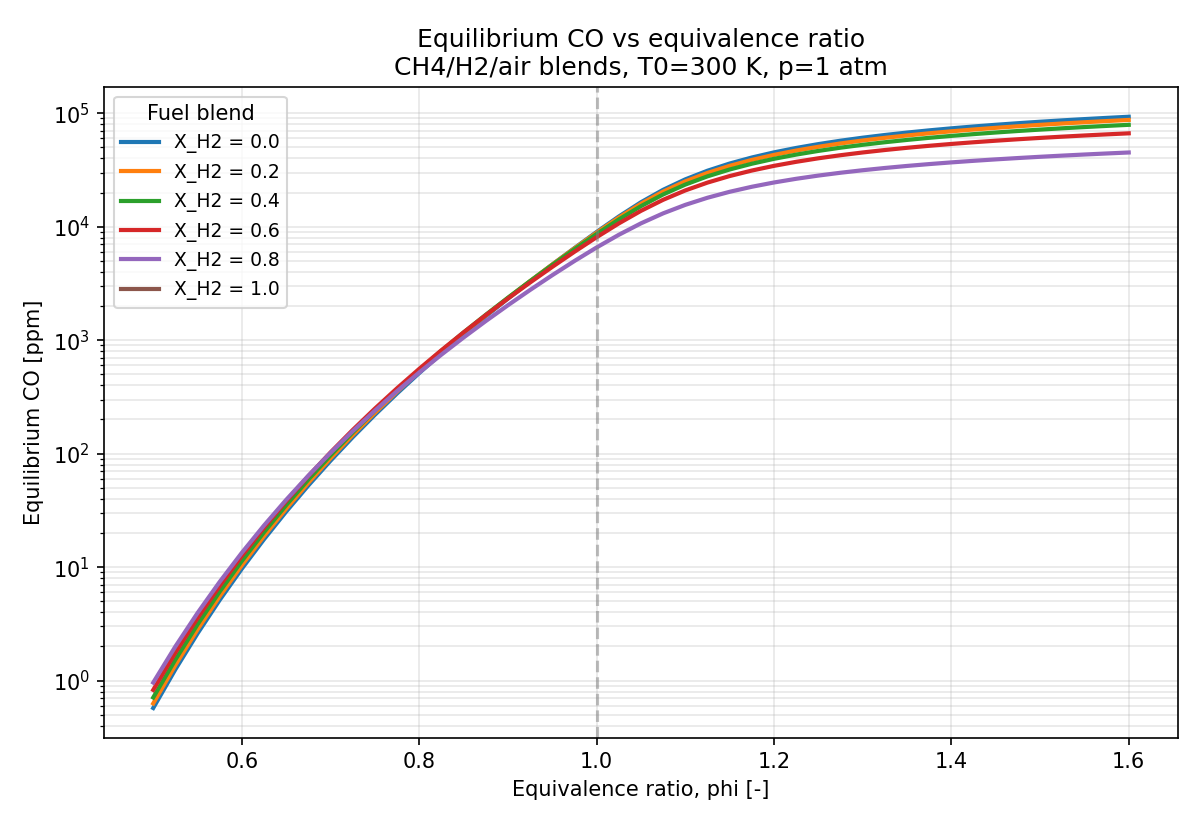
\includegraphics[width=0.85\textwidth]{03_equilibrium_CO_vs_phi.png}
    \caption{Equilibrium CO vs equivalence ratio for \ch{CH4}/\ch{H2}/air blends.}
    \label{fig:co_phi}
\end{figure}

Figure~\ref{fig:noxco_xh2} shows NO\textsubscript{x} and \ch{CO} as a function of $X_{H2}$ for three equivalence ratios
($\phi=0.8$, $1.0$, $1.2$). Several trends are visible:
\begin{itemize}
    \item \textbf{NO\textsubscript{x}} increases monotonically with $X_{H2}$ at all three equivalence ratios. The lean
    mixture ($\phi=0.8$) has the highest absolute NO\textsubscript{x} levels (\SI{1888.6}{ppm} to \SI{4322.8}{ppm} as
    $X_{H2}$ goes from 0 to 1) -- higher than at $\phi=1.0$ -- despite having a \emph{lower} flame temperature
    (e.g. $T_{ad}=\SI{1996.9}{K}$ at $\phi=0.8,X_{H2}=0$ vs $T_{ad}=\SI{2225.5}{K}$ at $\phi=1.0,X_{H2}=0$). This
    apparent contradiction is explained by the equilibrium \ch{O2} availability: thermal \ch{NO} formation
    (\ch{N2 + O <=> NO + N}, \ch{N + O2 <=> NO + O}) requires free \ch{O} and \ch{O2}, which are abundant under
    lean conditions but nearly absent at $\phi=1.2$. The relative NO\textsubscript{x} increase with $X_{H2}$ is largest for
    the rich mixture ($\phi=1.2$: from \SI{117.4}{ppm} to \SI{500.7}{ppm}, a factor of $\sim$4.3), because the
    higher H/O ratio of the hydrogen-rich blend leaves more residual \ch{O2}/\ch{O} available even under
    globally fuel-rich conditions.
    \item \textbf{\ch{CO}} decreases monotonically with $X_{H2}$ for $\phi=1.0$ and $\phi=1.2$ (reaching exactly
    zero at $X_{H2}=1$), as discussed above. At $\phi=0.8$, \ch{CO} is non-monotonic, rising slightly with
    $X_{H2}$ up to about $X_{H2}\approx0.6$ (from \SI{514.2}{ppm} to \SI{559.3}{ppm}) before falling sharply to
    zero -- a consequence of the higher flame temperature at larger $X_{H2}$ promoting \ch{CO2} dissociation back
    to \ch{CO}, until the diminishing amount of carbon in the blend dominates.
\end{itemize}

\begin{figure}[H]
    \centering
    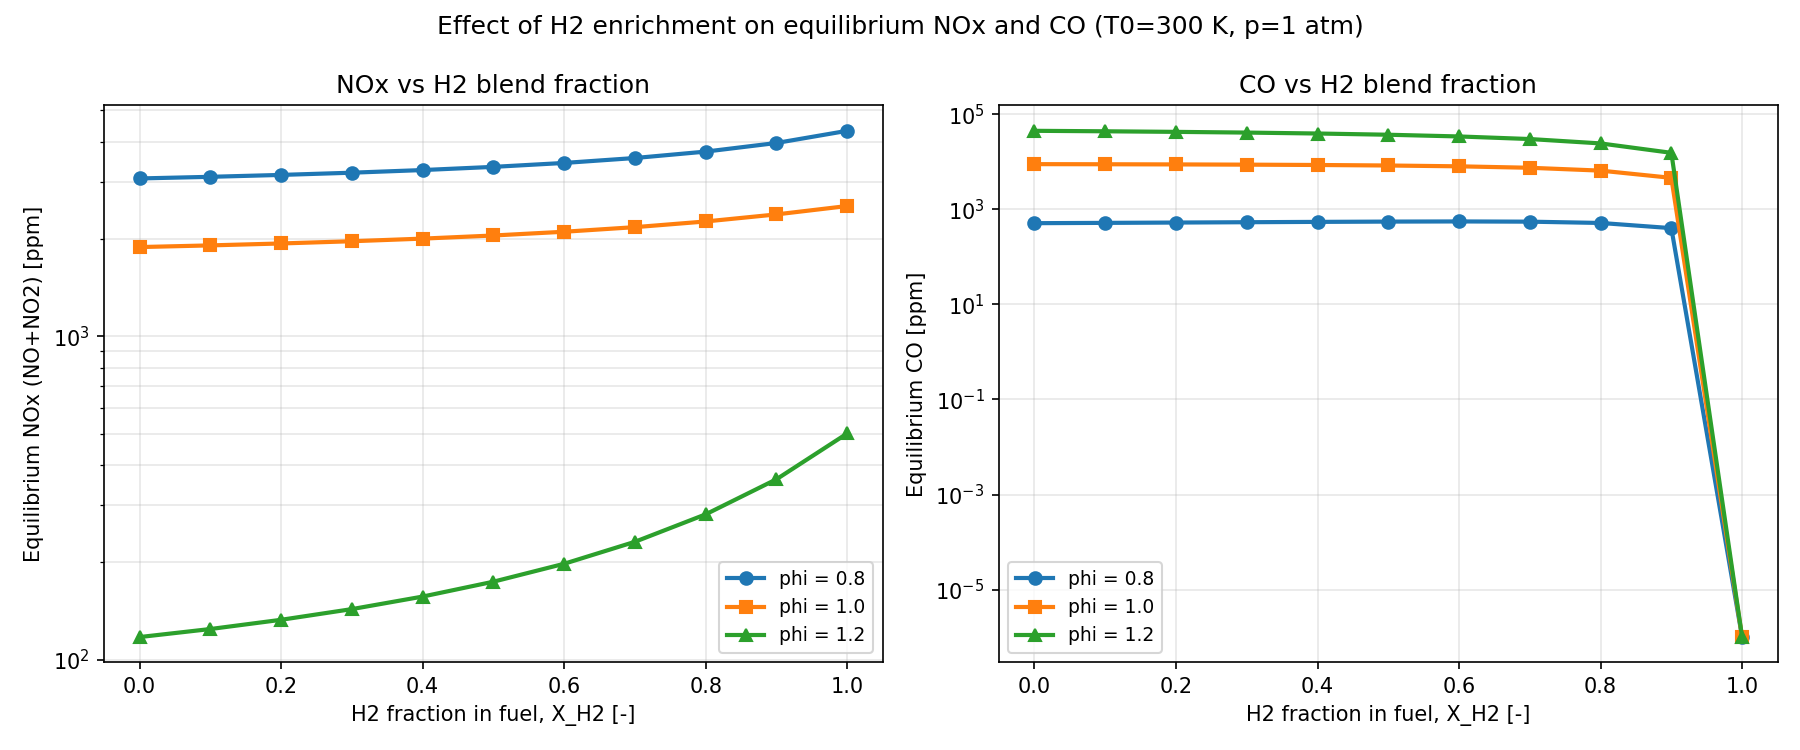
\includegraphics[width=\textwidth]{04_NOx_CO_vs_xH2.png}
    \caption{Equilibrium NO\textsubscript{x} and CO vs hydrogen blend fraction $X_{H2}$, for $\phi=0.8$, $1.0$ and $1.2$.}
    \label{fig:noxco_xh2}
\end{figure}

\subsection{Laminar flame speed}
\label{sec:flame_speed}

Figure~\ref{fig:sl_phi} shows the laminar flame speed $S_L$ as a function of equivalence ratio for the five fuel
blends $X_{H2} \in \{0, 0.25, 0.5, 0.75, 1.0\}$. For all blends, $S_L$ peaks on the slightly rich side of
stoichiometric ($\phi \approx 1.0$--$1.15$), consistent with the well-known behaviour of hydrocarbon and hydrogen
flames. The peak flame speed increases strongly and increasingly steeply with $X_{H2}$:

\begin{table}[H]
\centering
\caption{Laminar flame speed $S_L$ [cm/s] vs equivalence ratio and hydrogen fraction ($T_0=\SI{300}{K}$, $p=\SI{1}{atm}$).}
\label{tab:sl_phi}
\begin{tabular}{cccccc}
\toprule
$X_{H2}$ & $\phi=0.70$ & $\phi=0.85$ & $\phi=1.00$ & $\phi=1.15$ & $\phi=1.30$ \\
\midrule
0.00 & 19.6  & 31.3  & 38.5  & 37.1  & 23.9 \\
0.25 & 23.4  & 37.3  & 46.1  & 45.7  & 32.4 \\
0.50 & 30.6  & 48.3  & 60.7  & 63.1  & 50.6 \\
0.75 & 47.7  & 75.3  & 97.9  & 108.8 & 102.2 \\
1.00 & 122.0 & 185.2 & 234.0 & 270.0 & 294.2 \\
\bottomrule
\end{tabular}
\end{table}

\begin{figure}[H]
    \centering
    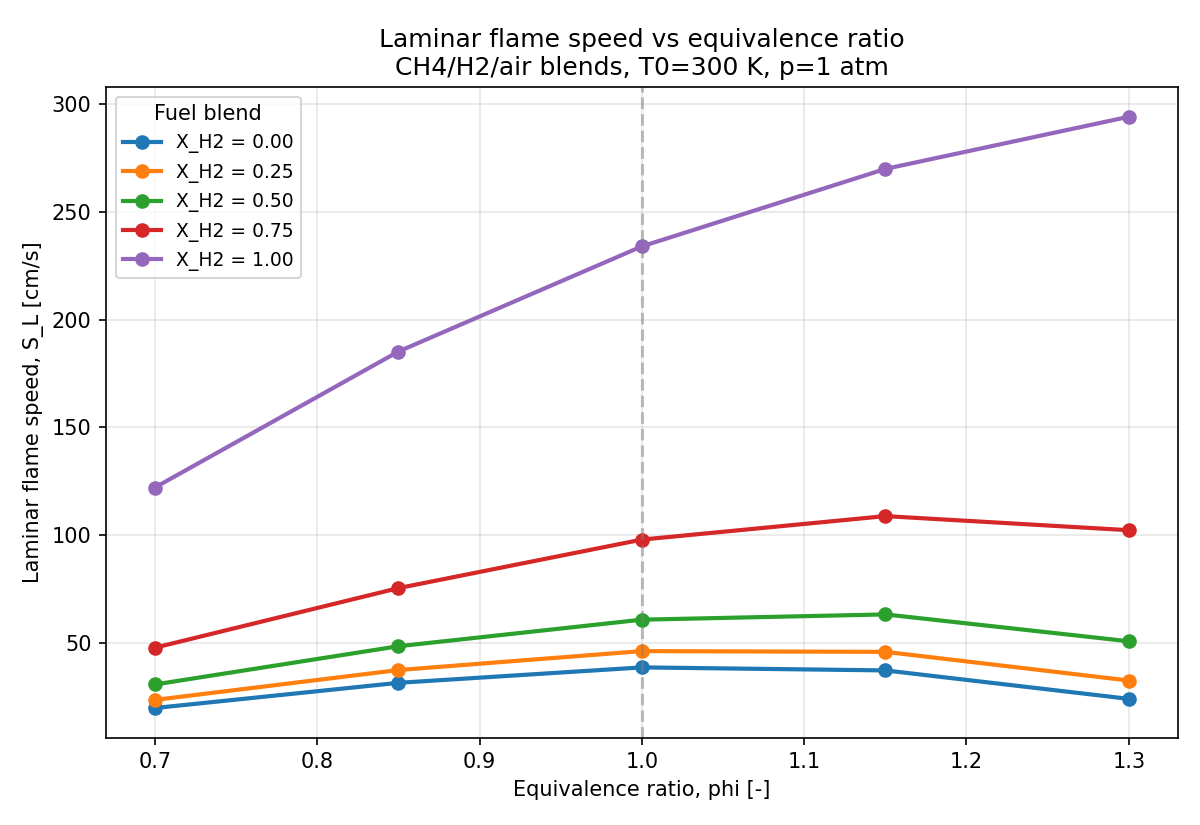
\includegraphics[width=0.85\textwidth]{05_SL_vs_phi.png}
    \caption{Laminar flame speed vs equivalence ratio for \ch{CH4}/\ch{H2}/air blends.}
    \label{fig:sl_phi}
\end{figure}

The pure-methane value $S_L\approx\SI{38.5}{cm/s}$ at $\phi=1.0$ agrees well with the commonly quoted experimental
range of \SIrange{36}{40}{cm/s} for methane--air flames at atmospheric conditions. Two effects are particularly
notable:

\begin{itemize}
    \item The flame speed increase with $X_{H2}$ is strongly \emph{nonlinear}: at $\phi=1.0$, going from $X_{H2}=0$
    to $0.5$ roughly increases $S_L$ from \SI{38.5}{} to \SI{60.7}{cm/s} (a 1.6-fold increase), while going from
    $X_{H2}=0.5$ to $1.0$ increases $S_L$ from \SI{60.7}{} to \SI{234.0}{cm/s} (a 3.9-fold increase) -- an overall
    increase of about a factor of 6 from pure methane to pure hydrogen. This is shown explicitly in
    Figure~\ref{fig:sl_xh2}, where the steepest rise occurs above $X_{H2}\approx0.5$. The dominant cause is the very
    high diffusivity of \ch{H2} and the increasing role of the chain-branching reaction
    \ch{H + O2 -> OH + O}, whose rate increases superlinearly as \ch{H2} becomes a larger fraction of the fuel.
    \item The location of the peak $S_L$ shifts toward richer mixtures as $X_{H2}$ increases: for $X_{H2}=0$ the
    peak is near $\phi\approx1.0$, whereas for $X_{H2}=1$ the flame speed is still increasing at $\phi=1.30$ (the
    richest case considered), consistent with the well-known shift of the peak burning velocity of hydrogen--air
    flames to $\phi\approx1.6$--$1.8$ due to preferential diffusion effects.
\end{itemize}

\begin{figure}[H]
    \centering
    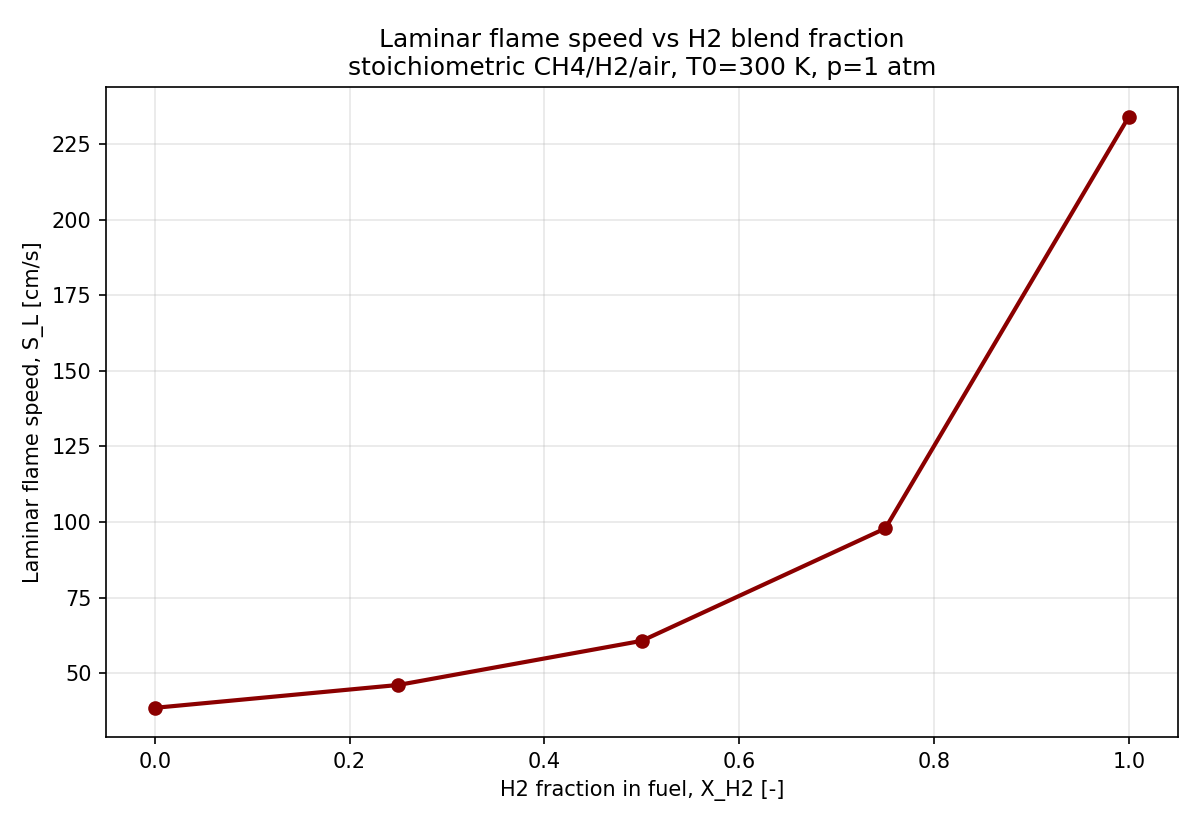
\includegraphics[width=0.85\textwidth]{06_SL_vs_xH2.png}
    \caption{Laminar flame speed vs hydrogen blend fraction $X_{H2}$ at stoichiometric conditions ($\phi=1.0$).}
    \label{fig:sl_xh2}
\end{figure}

Figure~\ref{fig:sl_pressure} shows the effect of pressure on $S_L$ at stoichiometric conditions for
$X_{H2}\in\{0,0.5,1.0\}$, over $p \in \{1,3,6\}$~bar:

\begin{table}[H]
\centering
\caption{Laminar flame speed $S_L$ [cm/s] vs pressure at $\phi=1.0$, $T_0=\SI{300}{K}$.}
\label{tab:sl_p}
\begin{tabular}{cccc}
\toprule
$X_{H2}$ & $p=\SI{1}{bar}$ & $p=\SI{3}{bar}$ & $p=\SI{6}{bar}$ \\
\midrule
0.00 & 38.7  & 24.8  & 17.7 \\
0.50 & 61.0  & 39.6  & 28.5 \\
1.00 & 234.0 & 215.8 & 181.7 \\
\bottomrule
\end{tabular}
\end{table}

For all three blends, $S_L$ decreases with increasing pressure, in agreement with the classical
$S_L \propto p^{n-1}$ scaling for an overall reaction order $n<1$ (typically $n\approx1.6$--$1.8$ for hydrocarbon
and hydrogen flames, giving $n-1<0$). However, the \emph{relative} sensitivity to pressure differs markedly between
the blends: from 1 to 6 bar, $S_L$ for pure methane drops by about 54\% (38.7 $\to$ 17.7 cm/s), whereas for pure
hydrogen it drops by only about 22\% (234.0 $\to$ 181.7 cm/s). This is consistent with the higher overall reaction
order (closer to 2) typically reported for hydrogen flames compared with methane flames, making hydrogen flame
speed comparatively more robust to pressure increase -- a relevant consideration for pressurized combustion systems
(e.g. gas turbines) operating on hydrogen-enriched fuel.

\begin{figure}[H]
    \centering
    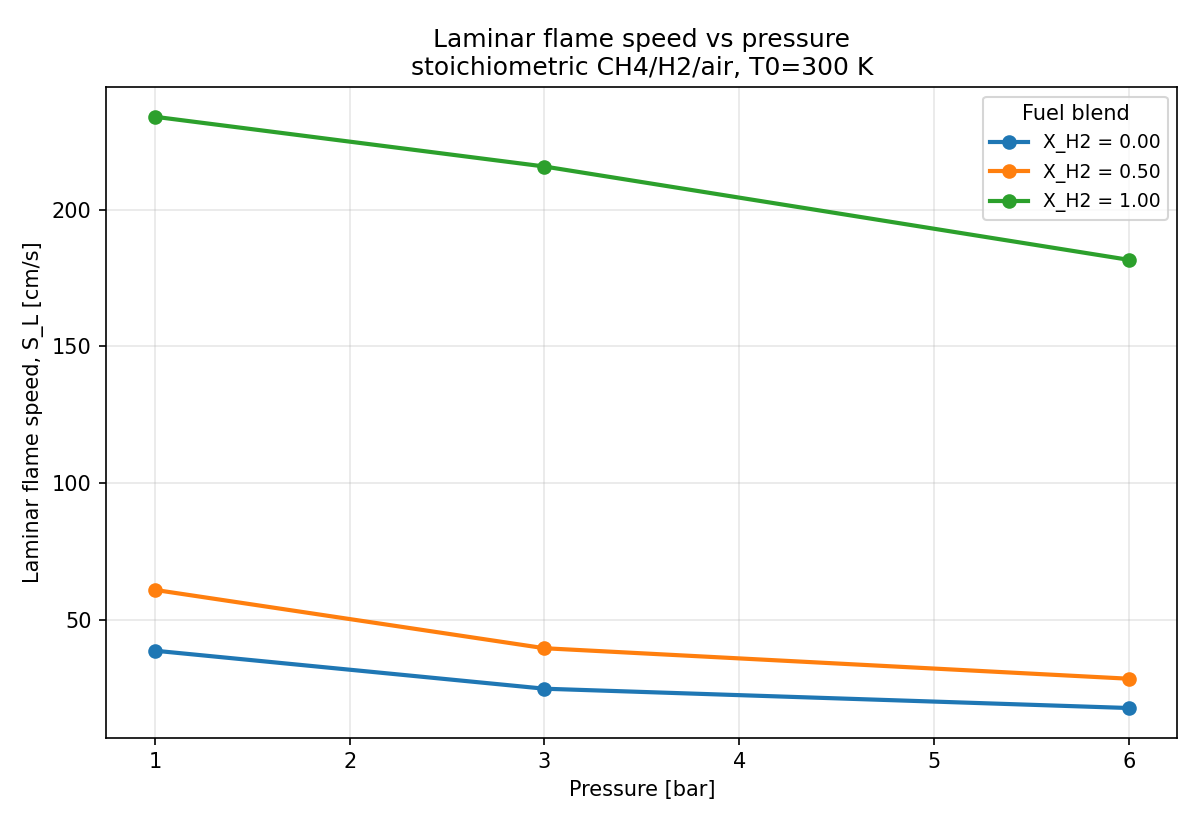
\includegraphics[width=0.85\textwidth]{07_SL_vs_pressure.png}
    \caption{Laminar flame speed vs pressure at $\phi=1.0$ for $X_{H2}=0$, $0.5$ and $1.0$.}
    \label{fig:sl_pressure}
\end{figure}

Finally, Figure~\ref{fig:structure} shows the spatial structure (temperature and major species mole fractions) of
the stoichiometric $X_{H2}=0.5$ flame. The computed burned-gas temperature ($T\approx\SI{2260}{K}$) matches the
equilibrium adiabatic flame temperature for the same composition (\SI{2258.4}{K}, Section~\ref{sec:equilibrium}) to
within 0.1\%, confirming the consistency between the equilibrium and 1D flame models. The reaction zone is only a
fraction of a millimetre thick, with \ch{OH} -- a marker of the high-temperature reaction zone -- peaking sharply
at the location where \ch{CH4} and \ch{H2} are simultaneously consumed.

\begin{figure}[H]
    \centering
    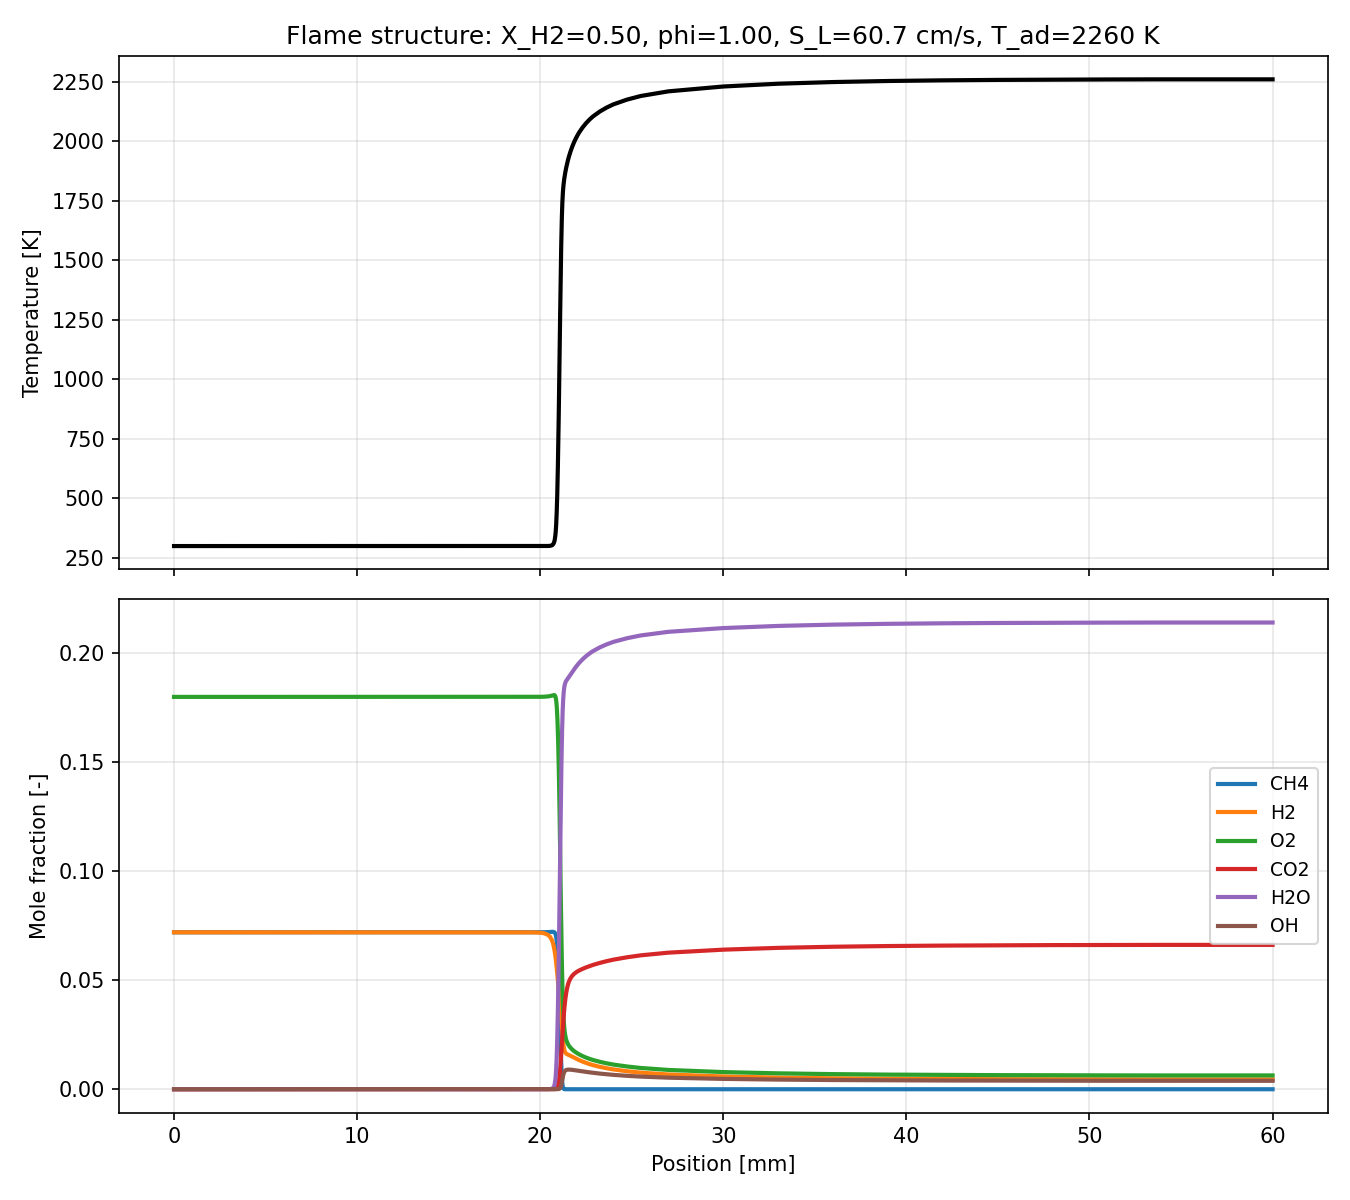
\includegraphics[width=0.85\textwidth]{08_flame_structure.png}
    \caption{Flame structure (temperature and major species mole fractions) for the stoichiometric $X_{H2}=0.5$ flame.}
    \label{fig:structure}
\end{figure}

\subsection{Ignition delay}
\label{sec:ignition}

Figure~\ref{fig:arrhenius} shows the ignition delay time $\tau$ as a function of $1000/T_0$ (an Arrhenius-type
representation) at $p_0=\SI{10}{bar}$, $\phi=1.0$, for the five fuel blends. As expected, $\tau$ decreases
approximately exponentially with increasing $T_0$ for all blends (an approximately straight line on the
semi-logarithmic plot), reflecting the Arrhenius temperature dependence of the dominant chain-branching reaction
rate. At every temperature, increasing $X_{H2}$ reduces $\tau$, and the effect is dramatic:

\begin{table}[H]
\centering
\caption{Ignition delay time $\tau$ [ms] vs initial temperature $T_0$ and hydrogen fraction ($p_0=\SI{10}{bar}$, $\phi=1.0$).}
\label{tab:tau_T0}
\begin{tabular}{cccccc}
\toprule
$T_0$ [K] & $X_{H2}=0.00$ & $X_{H2}=0.25$ & $X_{H2}=0.50$ & $X_{H2}=0.75$ & $X_{H2}=1.00$ \\
\midrule
900  & 594.4  & 165.7  & 158.6  & 137.3  & 101.8  \\
1000 & 80.9   & 12.85  & 11.49  & 10.20  & 8.106  \\
1100 & 16.98  & 1.737  & 1.154  & 0.9807 & 0.8342 \\
1200 & 4.528  & 0.4906 & 0.1954 & 0.1036 & 0.06067\\
1400 & 0.4721 & 0.1027 & 0.03332& 0.01066& 0.002284\\
\bottomrule
\end{tabular}
\end{table}

At $T_0=\SI{1100}{K}$, adding just 25\% \ch{H2} (by mole, in the fuel) already reduces $\tau$ from \SI{16.98}{ms} to
\SI{1.737}{ms} -- nearly a 10-fold reduction -- while the further reduction from $X_{H2}=0.25$ to $X_{H2}=1.0$
($1.737\to0.834$~ms) is comparatively modest. The same pattern (a very steep drop from $X_{H2}=0$ to $\approx0.25$,
followed by a much shallower decrease) is visible across the whole temperature range and is shown explicitly in
Figure~\ref{fig:tau_xh2}. This indicates that even a relatively small admixture of hydrogen into methane has a
disproportionately large effect on the auto-ignition propensity of the blend -- an important safety consideration
for hydrogen-blending in gas networks and combustion systems originally designed for pure methane.

\begin{figure}[H]
    \centering
    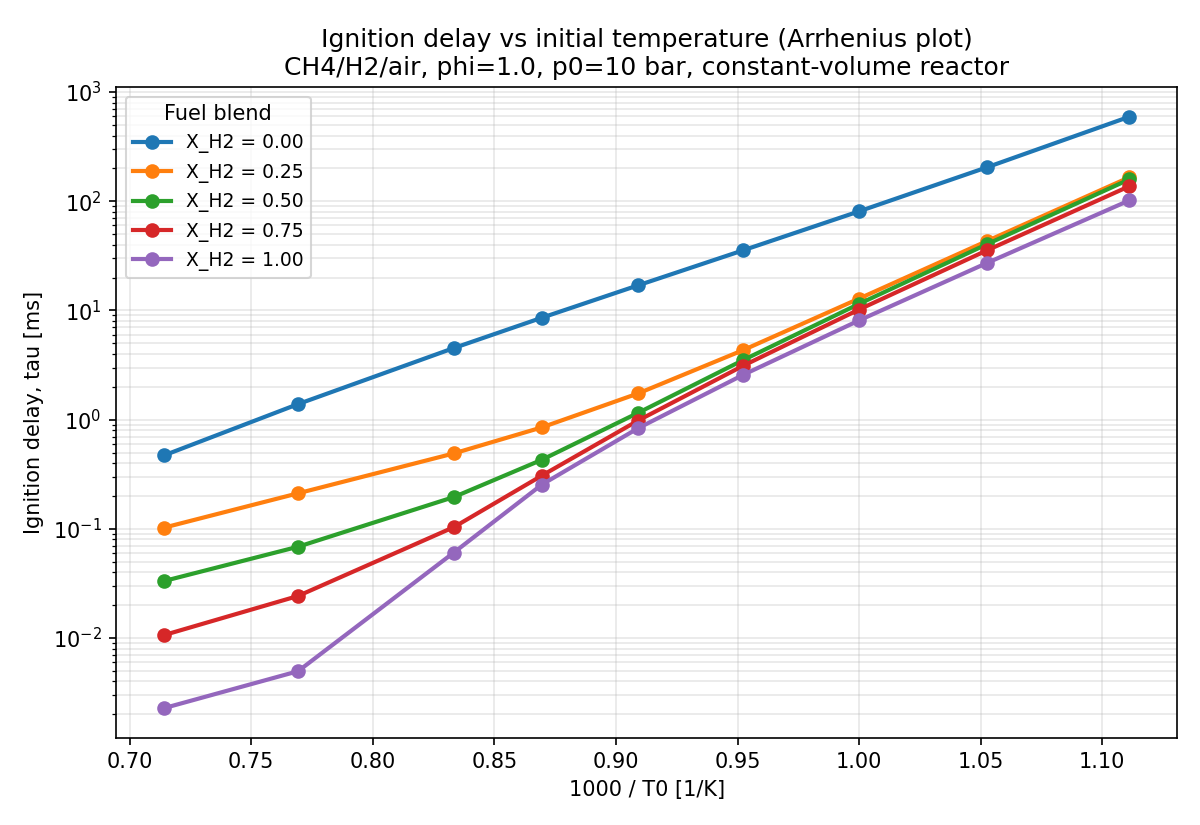
\includegraphics[width=0.85\textwidth]{09_ignition_delay_Arrhenius.png}
    \caption{Ignition delay time vs $1000/T_0$ (Arrhenius plot) at $p_0=\SI{10}{bar}$, $\phi=1.0$.}
    \label{fig:arrhenius}
\end{figure}

\begin{figure}[H]
    \centering
    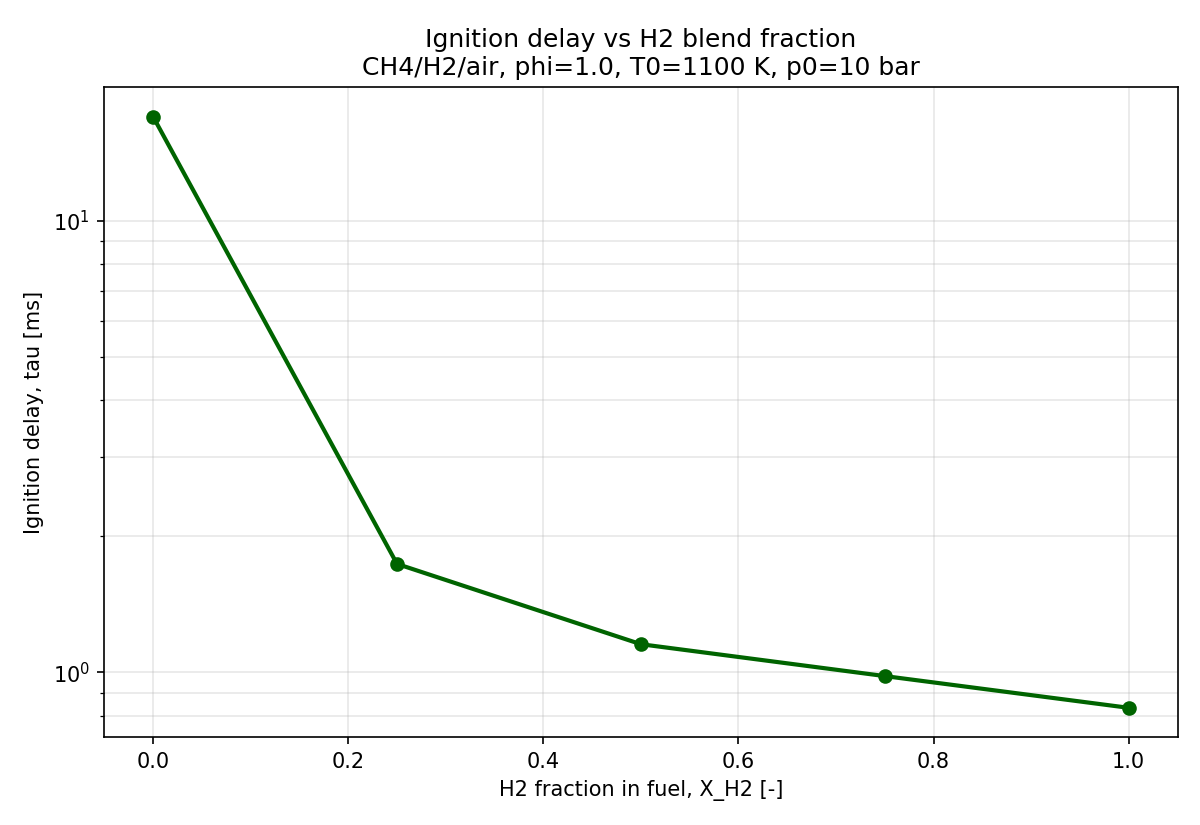
\includegraphics[width=0.85\textwidth]{11_ignition_delay_vs_xH2.png}
    \caption{Ignition delay time vs hydrogen blend fraction $X_{H2}$ at $T_0=\SI{1100}{K}$, $p_0=\SI{10}{bar}$, $\phi=1.0$.}
    \label{fig:tau_xh2}
\end{figure}

Figure~\ref{fig:tau_p} and Table~\ref{tab:tau_p} show the pressure dependence of $\tau$ at $T_0=\SI{1100}{K}$ for
$X_{H2}\in\{0,0.5,1.0\}$:

\begin{table}[H]
\centering
\caption{Ignition delay time $\tau$ [ms] vs initial pressure $p_0$ at $T_0=\SI{1100}{K}$, $\phi=1.0$.}
\label{tab:tau_p}
\begin{tabular}{cccc}
\toprule
$X_{H2}$ & $p_0=\SI{1}{bar}$ & $p_0=\SI{10}{bar}$ & $p_0=\SI{25}{bar}$ \\
\midrule
0.00 & 200.4   & 16.98  & 6.101 \\
0.50 & 2.001   & 1.154  & 0.9594\\
1.00 & 0.08702 & 0.8342 & 0.6643\\
\bottomrule
\end{tabular}
\end{table}

For pure methane ($X_{H2}=0$), $\tau$ decreases monotonically with pressure (200.4 $\to$ 16.98 $\to$ \SI{6.101}{ms}
from 1 to 25 bar), as expected for a chain-branching system where increased pressure increases the collision/
reaction rates. However, for pure hydrogen ($X_{H2}=1$), the trend is qualitatively \emph{opposite} at low
pressure: $\tau$ \emph{increases} by almost an order of magnitude from 1 to 10 bar (0.087 $\to$ \SI{0.834}{ms})
before decreasing again from 10 to 25 bar (0.834 $\to$ \SI{0.664}{ms}). The $X_{H2}=0.5$ blend shows an intermediate,
much weaker version of the same non-monotonic behaviour (2.00 $\to$ 1.15 $\to$ \SI{0.959}{ms}).

\begin{figure}[H]
    \centering
    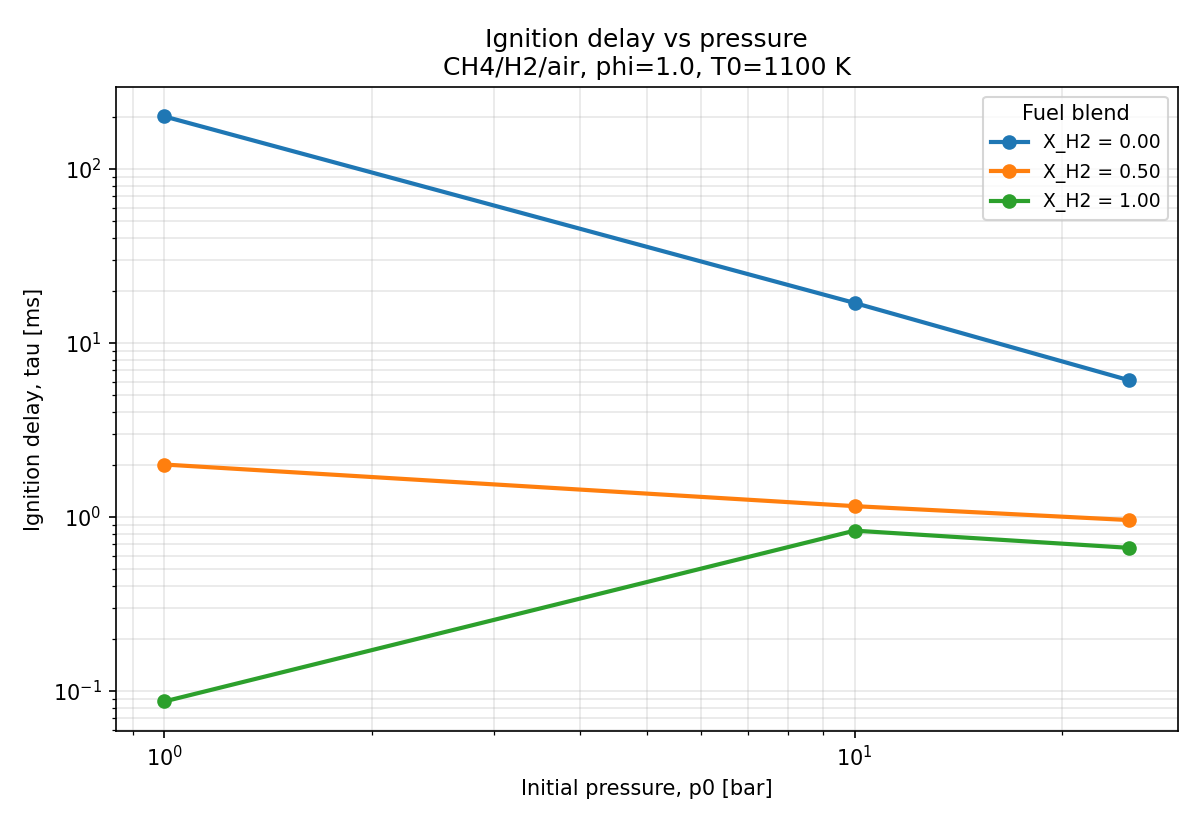
\includegraphics[width=0.85\textwidth]{10_ignition_delay_vs_pressure.png}
    \caption{Ignition delay time vs pressure at $T_0=\SI{1100}{K}$, $\phi=1.0$, for $X_{H2}=0$, $0.5$ and $1.0$.}
    \label{fig:tau_p}
\end{figure}

This non-monotonic behaviour for hydrogen-rich mixtures is a well-documented consequence of the competition between
two reactions involving the \ch{H} radical \cite{donohoe2014}:
\begin{align}
    &\ch{H + O2 -> OH + O} && \text{(chain branching, pressure-independent)} \\
    &\ch{H + O2 + M -> HO2 + M} && \text{(chain terminating, third-order, } \propto p^2 \text{)}
\end{align}
The first reaction produces two reactive radicals (\ch{OH} and \ch{O}) from one \ch{H} atom and drives the chain
reaction forward; the second consumes an \ch{H} radical to form the comparatively unreactive \ch{HO2}, removing
radicals from the branching chain. Because the second reaction is third-order, its rate grows with the square of
the pressure, while the first reaction's rate is pressure-independent. At low pressure, branching dominates and
increasing pressure increases the overall reaction rate (shorter $\tau$); but for fuels whose ignition chemistry is
dominated by the \ch{H}/\ch{O2} system (i.e. hydrogen-rich blends), there is a pressure range where the growth of
the termination reaction outpaces the branching reaction, causing the net radical pool to grow more slowly and
$\tau$ to \emph{increase} with pressure -- the "ignition delay turnover" behaviour seen here for $X_{H2}=1$ between 1
and 10 bar. For methane, the larger relative contribution of \ch{CH4}-specific branching pathways (which do not
involve this particular three-body step in the same way) means the overall ignition delay remains monotonically
decreasing with pressure over the range studied.

%======================================================================
\section{Conclusions}
%======================================================================

A systematic numerical study of \ch{CH4}/\ch{H2}/air combustion was carried out using the GRI-Mech 3.0 mechanism in
Cantera, covering chemical equilibrium, one-dimensional laminar premixed flames, and zero-dimensional auto-ignition,
for hydrogen blend fractions $X_{H2}$ from 0 (pure methane) to 1 (pure hydrogen). The main findings are:

\begin{enumerate}
    \item \textbf{Adiabatic flame temperature} increases monotonically with $X_{H2}$, from a maximum of
    \SI{2233.2}{K} (pure \ch{CH4}, $\phi\approx1.02$) to \SI{2396.3}{K} (pure \ch{H2}, $\phi\approx1.08$), with the
    peak shifting slightly toward richer mixtures as $X_{H2}$ increases.
    \item \textbf{Equilibrium NO\textsubscript{x}} increases monotonically with $X_{H2}$ at all equivalence ratios studied
    (e.g. by $\sim$34\% at $\phi=1.0$, from 1888.6 to 2529.5 ppm), tracking the increase in flame temperature.
    Counter-intuitively, lean mixtures ($\phi=0.8$) show \emph{higher} equilibrium NO\textsubscript{x} than stoichiometric
    mixtures despite lower flame temperatures, because of the much higher residual \ch{O2}/\ch{O} concentration
    available to drive thermal \ch{NO} formation.
    \item \textbf{Equilibrium \ch{CO}} decreases (toward zero) with increasing $X_{H2}$ at stoichiometric and rich
    conditions, simply reflecting the reduced carbon content of the fuel blend, but shows a slight non-monotonic
    increase at lean conditions before falling to zero.
    \item \textbf{Laminar flame speed} increases strongly and nonlinearly with $X_{H2}$ -- by a factor of
    $\sim$6 at stoichiometric conditions, from \SI{38.5}{cm/s} (pure \ch{CH4}) to \SI{234.0}{cm/s} (pure \ch{H2}) --
    with the steepest increase occurring for $X_{H2}\gtrsim0.5$. The location of peak $S_L$ shifts toward richer
    mixtures with increasing $X_{H2}$.
    \item \textbf{Pressure sensitivity of $S_L$} is markedly different between fuels: from 1 to 6 bar, pure
    methane's flame speed drops by $\sim$54\% while pure hydrogen's drops by only $\sim$22\%, making
    hydrogen-enriched flames comparatively more robust at elevated pressure.
    \item \textbf{Ignition delay} decreases dramatically with $X_{H2}$, with the largest relative effect occurring
    already for small hydrogen additions ($X_{H2}=0\to0.25$ gives nearly a 10-fold reduction at $T_0=\SI{1100}{K}$,
    $p_0=\SI{10}{bar}$); further increases in $X_{H2}$ have a comparatively smaller effect.
    \item \textbf{Pressure dependence of ignition delay} is qualitatively different between fuels: monotonically
    decreasing for pure methane, but non-monotonic (increasing then decreasing) for pure hydrogen, due to the
    competition between the pressure-independent chain-branching reaction \ch{H+O2->OH+O} and the third-order,
    pressure-squared chain-terminating reaction \ch{H+O2+M->HO2+M}.
\end{enumerate}

\subsection*{Practical implications}

These results illustrate that even moderate hydrogen blending into methane-fuelled systems can have
disproportionately large effects on key combustion characteristics -- particularly flame speed (affecting
flashback/blow-off limits of burners) and ignition delay (affecting auto-ignition safety margins and pre-ignition
risk in engines) -- well before $X_{H2}$ approaches 1. NO\textsubscript{x} emissions also increase steadily with hydrogen
content, which may partially offset the \ch{CO2} reduction benefits of hydrogen blending unless burner design is
adapted (e.g. via leaner operation or staged combustion).

\newpage
\bibliographystyle{unsrt}
\bibliography{references}

\end{document}
